% Created by tikzDevice version 0.12.3.1 on 2021-01-20 12:15:01
% !TEX encoding = UTF-8 Unicode
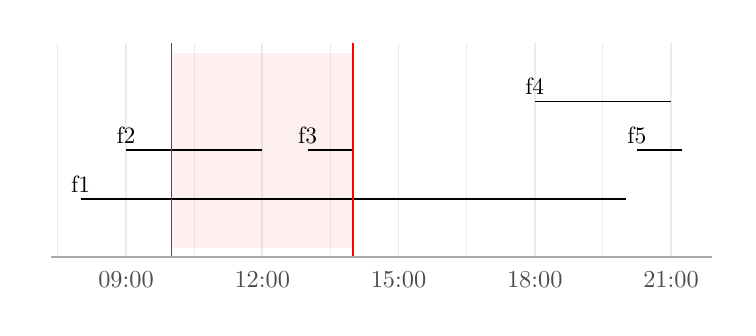
\begin{tikzpicture}[x=1pt,y=1pt]
\definecolor{fillColor}{RGB}{255,255,255}
\path[use as bounding box,fill=fillColor,fill opacity=0.00] (0,0) rectangle (252.94,101.18);
\begin{scope}
\path[clip] (  8.25, 18.22) rectangle (247.44, 95.68);
\definecolor{drawColor}{gray}{0.92}

\path[draw=drawColor,line width= 0.3pt,line join=round] ( 10.92, 18.22) --
	( 10.92, 95.68);

\path[draw=drawColor,line width= 0.3pt,line join=round] ( 60.15, 18.22) --
	( 60.15, 95.68);

\path[draw=drawColor,line width= 0.3pt,line join=round] (109.38, 18.22) --
	(109.38, 95.68);

\path[draw=drawColor,line width= 0.3pt,line join=round] (158.62, 18.22) --
	(158.62, 95.68);

\path[draw=drawColor,line width= 0.3pt,line join=round] (207.85, 18.22) --
	(207.85, 95.68);

\path[draw=drawColor,line width= 0.6pt,line join=round] ( 35.53, 18.22) --
	( 35.53, 95.68);

\path[draw=drawColor,line width= 0.6pt,line join=round] ( 84.77, 18.22) --
	( 84.77, 95.68);

\path[draw=drawColor,line width= 0.6pt,line join=round] (134.00, 18.22) --
	(134.00, 95.68);

\path[draw=drawColor,line width= 0.6pt,line join=round] (183.24, 18.22) --
	(183.24, 95.68);

\path[draw=drawColor,line width= 0.6pt,line join=round] (232.47, 18.22) --
	(232.47, 95.68);
\definecolor{fillColor}{RGB}{255,0,0}

\path[fill=fillColor,fill opacity=0.01] ( 51.95, 21.74) rectangle (117.59, 92.16);

\path[fill=fillColor,fill opacity=0.01] ( 51.95, 21.74) rectangle (117.59, 92.16);

\path[fill=fillColor,fill opacity=0.01] ( 51.95, 21.74) rectangle (117.59, 92.16);

\path[fill=fillColor,fill opacity=0.01] ( 51.95, 21.74) rectangle (117.59, 92.16);

\path[fill=fillColor,fill opacity=0.01] ( 51.95, 21.74) rectangle (117.59, 92.16);
\definecolor{drawColor}{RGB}{0,0,0}

\path[draw=drawColor,line width= 0.6pt,line join=round] ( 19.12, 39.35) -- (216.06, 39.35);

\path[draw=drawColor,line width= 0.6pt,line join=round] ( 35.53, 56.95) -- ( 84.77, 56.95);

\path[draw=drawColor,line width= 0.6pt,line join=round] (101.18, 56.95) -- (117.59, 56.95);

\path[draw=drawColor,line width= 0.6pt,line join=round] (183.24, 74.55) -- (232.47, 74.55);

\path[draw=drawColor,line width= 0.6pt,line join=round] (220.16, 56.95) -- (236.57, 56.95);

\node[text=drawColor,anchor=base,inner sep=0pt, outer sep=0pt, scale=  0.85] at ( 19.12, 41.69) {f1};

\node[text=drawColor,anchor=base,inner sep=0pt, outer sep=0pt, scale=  0.85] at ( 35.53, 59.29) {f2};

\node[text=drawColor,anchor=base,inner sep=0pt, outer sep=0pt, scale=  0.85] at (101.18, 59.29) {f3};

\node[text=drawColor,anchor=base,inner sep=0pt, outer sep=0pt, scale=  0.85] at (183.24, 76.90) {f4};

\node[text=drawColor,anchor=base,inner sep=0pt, outer sep=0pt, scale=  0.85] at (220.16, 59.29) {f5};
\definecolor{drawColor}{RGB}{255,0,0}

\path[draw=drawColor,line width= 0.6pt,line join=round] ( 51.95, 18.22) -- ( 51.95, 95.68);

\path[draw=drawColor,line width= 0.6pt,line join=round] (117.59, 18.22) -- (117.59, 95.68);
\end{scope}
\begin{scope}
\path[clip] (  0.00,  0.00) rectangle (252.94,101.18);
\definecolor{drawColor}{RGB}{169,169,169}

\path[draw=drawColor,line width= 0.6pt,line join=round] (  8.25, 18.22) --
	(247.44, 18.22);
\end{scope}
\begin{scope}
\path[clip] (  0.00,  0.00) rectangle (252.94,101.18);
\definecolor{drawColor}{gray}{0.30}

\node[text=drawColor,anchor=base,inner sep=0pt, outer sep=0pt, scale=  0.88] at ( 35.53,  7.21) {09:00};

\node[text=drawColor,anchor=base,inner sep=0pt, outer sep=0pt, scale=  0.88] at ( 84.77,  7.21) {12:00};

\node[text=drawColor,anchor=base,inner sep=0pt, outer sep=0pt, scale=  0.88] at (134.00,  7.21) {15:00};

\node[text=drawColor,anchor=base,inner sep=0pt, outer sep=0pt, scale=  0.88] at (183.24,  7.21) {18:00};

\node[text=drawColor,anchor=base,inner sep=0pt, outer sep=0pt, scale=  0.88] at (232.47,  7.21) {21:00};
\end{scope}
\end{tikzpicture}
